\begin{figure}[t]
\centering
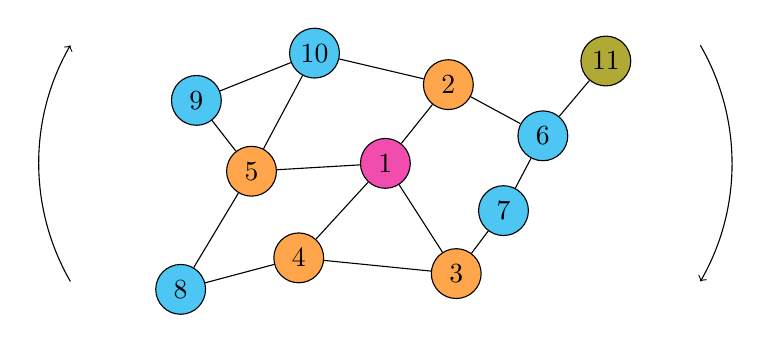
\begin{tikzpicture}
  \tikzstyle{node}=[circle,draw, minimum width=18pt, inner sep=0pt]
  \tikzstyle{root}=[fill=magenta!70]
  \tikzstyle{color1}=[fill=orange!70]
  \tikzstyle{color2}=[fill=cyan!70]
  \tikzstyle{color3}=[fill=olive!70]

  \node[node, root]   (1)  at (0,     0)    {$1$};
  \node[node, color1] (2)  at (0.8,   1)    {$2$};
  \node[node, color1] (3)  at (0.9,   -1.4) {$3$};
  \node[node, color1] (4)  at (-1.1,  -1.2) {$4$};
  \node[node, color1] (5)  at (-1.7,  -0.1) {$5$};
  \node[node, color2] (6)  at (1.5,   -0.6) {$7$};
  \node[node, color2] (7)  at (2,     0.35) {$6$};
  \node[node, color2] (8)  at (-0.9,  1.4)  {$10$};
  \node[node, color2] (9)  at (-2.4,  0.8)  {$9$};
  \node[node, color2] (10) at (-2.6,  -1.6) {$8$};
  \node[node, color3] (11) at (2.8,   1.3)  {$11$};

  \path (1) edge (2);
  \path (1) edge (3);
  \path (1) edge (4);
  \path (1) edge (5);
  \path (2) edge (7);
  \path (2) edge (8);
  \path (3) edge (4);
  \path (3) edge (6);
  \path (4) edge (10);
  \path (5) edge (8);
  \path (5) edge (9);
  \path (5) edge (10);
  \path (6) edge (7);
  \path (7) edge (11);
  \path (8) edge (9);

  \draw[<-] (4,  -1.5) arc (-30:30:3);
  \draw[<-] (-4, 1.5)  arc (150:210:3);
\end{tikzpicture}
\caption[Normalisierung für Graphen im zweidimensionalen Raum]{Normalisierung eines Receptive-Fields der Größe $11$ eines Graphen im zweidimensionalen euklidischen Raum.
  Knoten werden basierend \bzgl{} ihrer Pfadlänge zum Wurzelknoten (rot) gruppiert (dargestellt über die unterschiedlichen Farbtöne der Knoten).
  In diesen werden die Knoten entsprechend ihrer Winkel zum Wurzelknoten im Uhrzeigersinn geordnetet.}
\label{fig:normalisierung_erweitert}
\end{figure}
